\documentclass{article}
\usepackage[T1]{fontenc}
\usepackage[utf8]{inputenc}

\usepackage{cmbright}
\usepackage[T1]{fontenc}

\usepackage{multicol}

\usepackage{amsmath}
\usepackage{amsfonts}
\usepackage{amssymb}
\usepackage{tikz}
\usepackage{graphicx}
\graphicspath{  {./images/} }
\setlength{\parindent}{0pt}
\usepackage{changepage}
\usepackage{verbatim}
\usepackage{physics}
\usepackage{derivative}
\usepackage{bm}
\usepackage[colorlinks=true, linkcolor=blue, urlcolor=blue, citecolor=blue, anchorcolor=blue]{hyperref}

\addtolength{\oddsidemargin}{-.25in}
\addtolength{\textwidth}{0.5in}

\makeatletter
\newcommand*\bigcdot{\mathpalette\bigcdot@{.5}}
\newcommand*\bigcdot@[2]{\mathbin{\vcenter{\hbox{\scalebox{#2}{$\m@th#1\bullet$}}}}}
\makeatother

\DeclareMathOperator{\di}{d\!}
\newcommand*\Eval[3]{\left.#1\right\rvert_{#2}^{#3}}

\newcommand{\uvec}[1]{\boldsymbol{\hat{\textbf{#1}}}}
\newcommand{\vr}[1]{\textbf{#1}}

\newcommand{\thus}[0]{\; \; \longrightarrow \; \;}

\newcommand{\lag}{\mathcal{L}}
\newcommand{\ham}{\mathcal{H}}

\title{Mass Distribution Calculations}
\author{Ryan Liu}
\date{Last updated: July 23, 2021}

\begin{document}

\maketitle

\section{Resources Used}

\begin{itemize}
    \item V Tiwari, S Fairhurst. \textit{The Emergence of Structure in the Binary Black Hole Mass Distribution.} \url{https://arxiv.org/abs/2011.04502}
    \item LIGO Scientific Collaboration. \textit{Population Properties of Compact Objects from the Second Ligo-Virgo Gravitational Wave Transient Catalog.} \url{https://arxiv.org/abs/2010.14533}
    \item LIGO Scientific and VIRGO Collaborations. \textit{The basic physics of the binary black hole merger GW150914}. \url{https://arxiv.org/abs/1608.01940}
\end{itemize}

\section{Calculations}

The most important factor in determining the strength of a BBH GW signal is the component masses of the black holes. LIGO and other detectors often measure the \textit{chirp mass}, which is given by 
\begin{equation}
    \mathcal{M} = \frac{(m_1m_2)^{3/5}}{(m_1+m_2)^{1/5}} = \frac{c^3}{G} \Big( \Big(\frac{5}{96}\Big)^3 \pi^{-8} (f_{GW})^{-11}(\dot{f}_{GW})^3\Big)^{1/5}
\end{equation}
Determining the component masses from chirp mass introduces some imprecision as $\mathcal{M}_\text{meas.} = \mathcal{M}_0 (1+z)$. However, it is obvious that given the component masses $(m_1, m_2)$ or the primary mass and the mass ratio $(m_1, q)$, the chirp mass is easily computable. \\

Compared to the spin distribution, the mass distribution of BBH mergers has been determined with greater accuracy. As the mass distribution is determined empirically based on the results of iLIGO and aLIGO, they are only ``valid" for low redshifts ($z < 1$); however, for simplicity we \textbf{assume that the mass distribution of BBHs does not change as a function of redshift and is independent of the spin distribution}. \\

We consider two possible mass distributions: the \textbf{Broken Power Law} distribution and \textbf{Power Law + Peak} distribution, as described by Abbott et al., both of which are determined through 44 BBH observations from GWTC-1 and GWTC-2. We first introduce the \textit{smoothing function}, defined by 
\begin{equation}
    S(m_1 | m_{min}, \delta_m) = \begin{cases}
    0 & \text{if $m \leq m_{min}$} \\
    \Big[1 + \exp\Big(\frac{\delta_m}{m_1 - m_{min}} + \frac{\delta_m}{m_1-m_{min}-\delta_m} \Big) \Big]^{-1} & \text{if $m_{min} < m < m_{min} + \delta_m$} \\
    1 & \text{if $m \geq m_{min} + \delta_m$}
    \end{cases}
\end{equation}
We also denote the \textit{Gaussian distribution function} by 
\begin{equation}
    G(m_1 | \mu_m, \sigma_m) = \frac{1}{\sqrt{2\pi \sigma_m}} \exp \Big(\frac{-(m_1-\mu_m)^2}{2\sigma_m}\Big)
\end{equation}
and the \textit{power law function} by 
\begin{equation}
    P(m_1 | -\alpha, m_{min}, m_{max}) = \begin{cases}
    0 & \text{if $m < m_{min}$ or $m > m_{max}$} \\
    \frac{\alpha-1}{m_{min}} \frac{(x/m_{min})^{-\alpha}}{1-(m_{max}/m_{min})^{(1-\alpha)}} & \text{if $m_{min} < m < m_{max}$}
    \end{cases}
\end{equation}
The \textbf{Broken Power Law} distribution is therefore given by 
\begin{equation}
    \pi(m_1 | \alpha_1, \alpha_2, m_{min}, m_{max}, b) \propto \begin{cases}
    m_1^{-\alpha_1} S(m_1 | m_{min}, \delta_m) & \text{for $m_{min} < m_1 < m_{break}$} \\
    m_1^{-\alpha_2} S(m_1 | m_{min}, \delta_m) & \text{for $m_{break} < m_1 < m_{max}$}
    \end{cases}
\end{equation}
with 
\begin{equation}
    m_{break} = m_{min} + b(m_{max} - m_{min})
\end{equation}
and the accompanying mass ratio distribution 
\begin{equation}
    \pi(q \; | \; \beta_q, m_{min}, m_1) = q^{\beta_q} \text{  for $m_{min}/m_1 \leq q \leq 1$}
\end{equation}
The \textbf{Power Law + Peak} distribution is given by 
\begin{multline}
    \pi (m_1 | \lambda_{peak}, \alpha, m_{min}, m_{max}, \delta_m, \mu_m, \sigma_m) \\
    \propto \Big[ (1 - \lambda_{peak}) P(m_1 | -\alpha, m_{max}) + \lambda_{peak} G(m_1 | \mu_m, \sigma_m) \Big] S(m_1 | m_{min}, \delta_m)
\end{multline}
with the accompanying mass ratio distribution 
\begin{equation}
    \pi(q \; | \; \beta_q, m_1, m_{min}, \delta_m) \propto q^{\beta_q} S(qm_1 | m_{min}, \delta_m)
\end{equation}
Both of these distributions are designed to be more flexible in accommodating high-mass BBH mergers that do not fit well under a single truncated power law. Abbott et al. also uses a \textit{multi-peak} distribution which consists of an underlying power law distribution with multiple Gaussian peaks to test for hierarchial mergers; however, this model is not considered here. \\

For ease of calculation, we only use the median posterior for the two mass models. Furthermore, we note that both models are likely leaving out an important subpopulation of lower-end intermediate black holes ($m > 100 M_\odot$).

\newpage



\section{Results}

The median posteriors for the parameters of the Broken Power Law mass distribution are 
\begin{equation}
    \begin{gathered}
        \alpha_1 = 1.58, \quad \alpha_2 = 5.59, \quad \beta_q = 1.40, \quad \delta_m = 4.83 \\
        m_{min} = 3.96, \quad m_{max} = 87.14, \quad b = 0.43
    \end{gathered}
\end{equation}
and the median posteriors for the parameters of the Power Law + Peak distribution are 
\begin{equation}
    \begin{gathered}
        \alpha = 2.63, \quad \beta_q = 1.26, \quad \delta_m = 4.82, \quad m_{min} = 4.59 \\
        m_{max} = 86.22, \quad \lambda_{peak} = 0.10, \quad \mu_m = 33.07, \quad \sigma_m = 5.69
    \end{gathered}
\end{equation}
Using mass bins of $4 M_\odot$, we see in Figure \ref{fig:hist} that both distributions are similar, although the power law + peak model assigns a higher probability to high-mass BBHs. The mass ratio distribution is also very similar, although the power law + peak model includes a higher proportion of extreme mass ratios. \\

\begin{figure}[!htb]
    \center{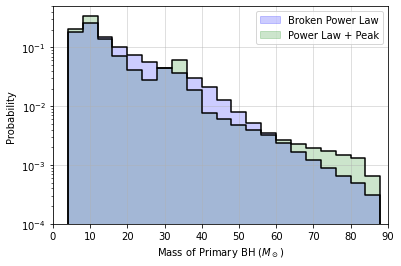
\includegraphics[width=2.5in]{SNR37.png}
    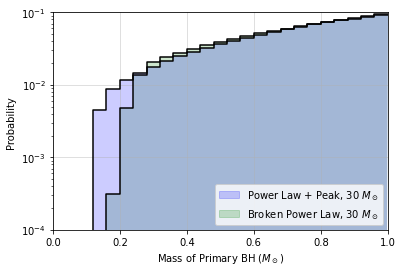
\includegraphics[width=2.5in]{SNR38.png}}
    \caption{\label{fig:hist} Probability density distribution of the (left) primary mass of BBH mergers using bins of $4 M_\odot$, starting at $m_{min} = 4 M_\odot$ and (right) mass ratio of BBH mergers with primary mass $30 M_\odot$ using bins of 0.04.}
\end{figure}

Combining both the primary mass and mass ratio distributions, we find as expected that the vast majority of the BBH population have low masses and are approximately symmetrical. These mergers generally produce longer GW signals with lower amplitudes, suggesting that even for Cosmic Explorer, the limiting factor in detection may remain to be signal amplitude, rather than the low frequency limit caused by redshift. 

\begin{figure}[!htb]
    \center{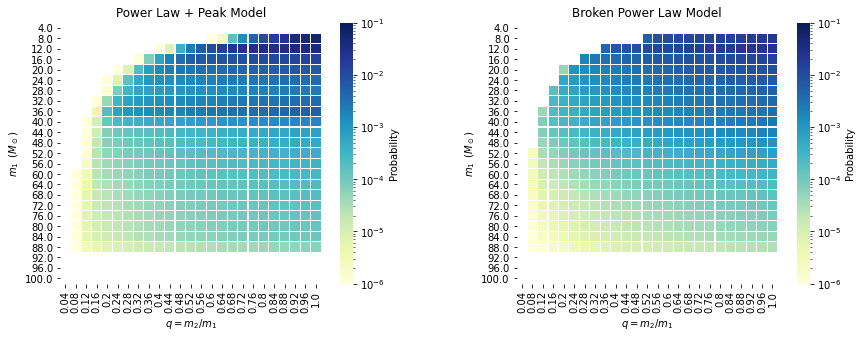
\includegraphics[width=\textwidth]{SNR39.png}}
    \caption{\label{fig:hist} Probability distribution of the BBH merger population across the entire $(m_1, q)$ range, in bins of $m_1 = 4 M_\odot$ and $q = 0.04$.}
\end{figure}

\begin{figure}[!htb]
    \center{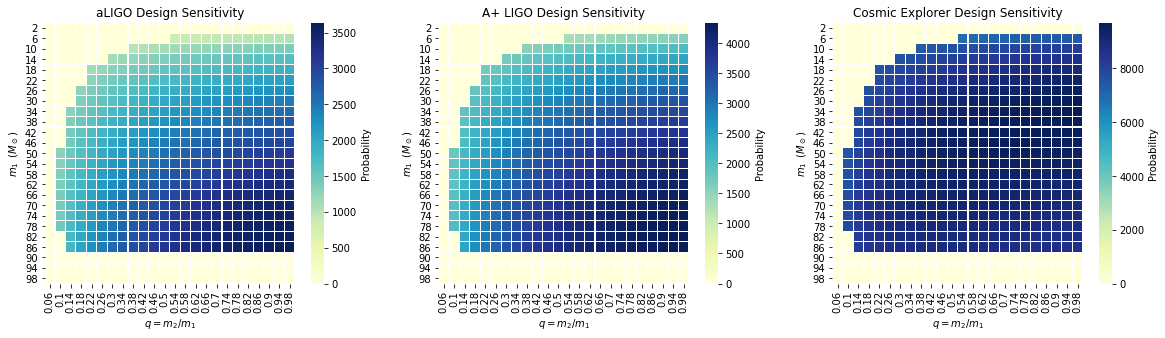
\includegraphics[width=\textwidth]{SNR40.png}}
    \caption{\label{fig:hist} Maximum comoving distance of observation for zero-spin BBHs over the full mass distribution (Broken Power Law model).}
\end{figure}













\end{document}